\chapter{中間発表までの主な活動}

\section{ブレインストーミング}
まず各々がこのチームで開発したいアイディアを,Miro\footnote{https://miro.com/}を使用して,書き出した.アイディアの例は以下である.

\begin{quote}
    \begin{itemize}
        \item 独り言を自動的に録音してテキスト化
        \item 健康促進アプリ(地図上でこれまで行った場所を塗りつぶす)
        \item 悩みがある人同士で会話できるもの
        \item 店など様々な場所の混雑度チェックアプリ
        \item 公共交通機関を携帯からリアルタイムに把握する
        \item 1日を可視化
    \end{itemize}
\end{quote}

各々違う色の付箋を使用し,KJ法を使用し意見をまとめた.この活動ではさまざまな意見が挙げられたが,一番チームの共感を得たバスについて,今後の活動を絞った.

\begin{figure}[htbp]
    \centering
    \includegraphics[width=9cm]{images/brainstorm.png}
    \caption{ブレインストーミング}
    \label{fig:brainstorm}
\end{figure}
\bunseki{大津武琉}

\section{アイディアの深掘り}

上記のブレインストーミングで挙げられたアイディアは煩雑なものであったため,実際に我々がバスを利用してきた中で不便に感じたことを考え,欲しい機能を列挙していった.機能の例は以下である.

\begin{quote}
    \begin{itemize}
        \item 交通系ICカードを取り込み残高を表示
        \item バス停までの徒歩時間表示
        \item バスの時刻表表示
        \item 地図上に表示するバスの数を変えれる
    \end{itemize}
\end{quote}

\begin{figure}[htbp]
    \centering
    \includegraphics[width=9cm]{images/dig.png}
    \caption{アイディアの深掘り}
    \label{fig:dig}
\end{figure}
\bunseki{下村蒔里萌}


\section{開発プラットフォームの決定}
まず,iOSとAndroidの2プラットフォームのネイティブアプリを並行して開発するか,クロスプラットフォームのネイティブアプリを開発するか,ということについて考えた.本グループでは2つの理由からクロスプラットフォーム開発に決定した.1つ目の理由は,グループの規模が小さいことである.プラットフォームを分けると,各プラットフォーム2〜3人となってしまい各人の負担が大きい.2つ目の理由は,本グループ全体の技術力が少ないことである.本グループには,過去に開発者としてアプリケーション開発を行ったことのある者が1人しかいない.ほかのメンバーは経験がなく,1から学習を始めるため,学習コストが大きい.以上の理由より,クロスプラットフォームのネイティブアプリの開発を進める形となった.使用するフレームワークはクロスプラットフォームの代表例であるFlutter\footnote{https://flutter.dev/}となった.
\bunseki{及川寛太}

\section{メンバーの役割決定}
本グループでは5人のメンバーで行っている.各メンバーの役割については以下の通りとなっている.

\subsection{プロダクトオーナー}
プロダクトオーナーはプロダクトの責任者であり,開発チームを活用して,そのプロダクトが生み出す価値を最大化する責任がある\cite{scrum}.
\begin{quote}
    \begin{itemize}
        \item 及川 寛太
    \end{itemize}
\end{quote}

\subsection{スクラムマスター}
スクラム開発を円滑に進める役割がある.具体的に,アジャイルとスクラムの価値を維持し,ほかの人がスクラムを理解し実践するのを助ける,スクラムのミーティングをファシリテートする \cite{scrummaster}.
\begin{quote}
    \begin{itemize}
        \item 大津 武琉
    \end{itemize}
\end{quote}

\subsection{デザイン}
問題やユーザ像の分析より,アプリのUXやUIを考え,Figma\footnote{https://www.figma.com/}でプロトタイプを作成する.実際にプログラムを書く際に必要な,レスポンシブな数値などのデザインシステムを作成する.
\begin{quote}
    \begin{itemize}
        \item 下村 蒔里萌
    \end{itemize}
\end{quote}

\subsection{iOSアプリ}
クロスプラットフォーム開発を行うが,iOS独自の開発が必要な場合や問題が発生した場合に,優先多岐に対応にあたる.
\begin{quote}
    \begin{itemize}
        \item 及川 寛太
        \item 下村 蒔里萌
    \end{itemize}
\end{quote}
\pagebreak
\subsection{Androidアプリ}
クロスプラットフォーム開発を行うが,Android独自の開発が必要な場合や問題が発生した場合に,優先多岐に対応にあたる.
\begin{quote}
    \begin{itemize}
        \item 大津 武琉
        \item 稲田敬介
        \item ディオガーディディラン基暉
    \end{itemize}
\end{quote}

\subsection{サーバ}
バスの運行に関わるデータの収集・記録・管理を行う.また,クライアント側が必要とする情報を素早く提供するシステムを開発する.
\begin{quote}
    \begin{itemize}
        \item 及川 寛太
        \item 大津 武琉
    \end{itemize}
\end{quote}
\bunseki{大津武琉}

\section{Git・GitHubの習得}
チーム開発を進める中で必要不可欠であるバージョン管理アプリのGitHub\footnote{https://github.com/}の勉強会を行なった.メンバーの過半数がGitHubを触ったことがなかったため,使用経験がある人から基本的な使用方法を教えてもらい,実際にGit\footnote{https://git-scm.com/}の機能であるClone,Commit,Push,Fetch,Merge,Pullを行なってGitHubについて学んだ.
\bunseki{ディオガーディディラン基暉}

\section{アプリ名の決定}
アプリの名前を考えることで,開発を進める上でのモチベーション維持を目指した.各々アプリ名を1つ以上考えることとなり以下のようなアプリ名が挙げられた.

\begin{quote}
    \begin{itemize}
        \item BuLo (ブーロ) : BusとLocationの頭をとったもので,美しく (Beautiful) ,有用なユーザーインターフェースUseful (UserInterface) を持つライブ (Live) で最良のオプション (Option) である.バスロケーションシステムという意味も持つ.
        \item Loco (ロコ) :「ロケーション」と「どこ」をかけたもの.
        \item nnuts (ナッツ) : No trouble with busの各単語から1文字とって組み合わせたもの.
        \item バスらく: バスをらくに使えるアプリを略したもの.横文字のアプリ名がたくさんあるが,ぱっと思い出しにくいため,名前からすぐにどんな用途かわかるものを提案した.
        \item ばすけん: バス検索を省略したもの.
    \end{itemize}
\end{quote}

上記のものでメンバー内で多数決をとった結果,BuLo (ブーロ) という名前に決定した.

\begin{figure}[htbp]
    \centering
    \includegraphics[width=9cm]{images/app_name.png}
    \caption{アプリ名案}
    \label{fig:app_name}
\end{figure}
\bunseki{稲田敬介}


\section{プロトタイプの作成}
イメージするアプリのプロトタイプをFigma\footnote{https://www.figma.com/}を用いて作成した (図2.4) .左から1枚目の画面は自分の現在地を表示させている.2〜4枚目は目的地を入力する画面となっている.5〜6枚目は現在地から2〜3枚目で入力した場所までのバスを表示させる.7枚目では5〜6枚目で選択したバスと自分との位置関係をグラフと地図で表示させる.

\begin{figure}[htbp]
    \centering
    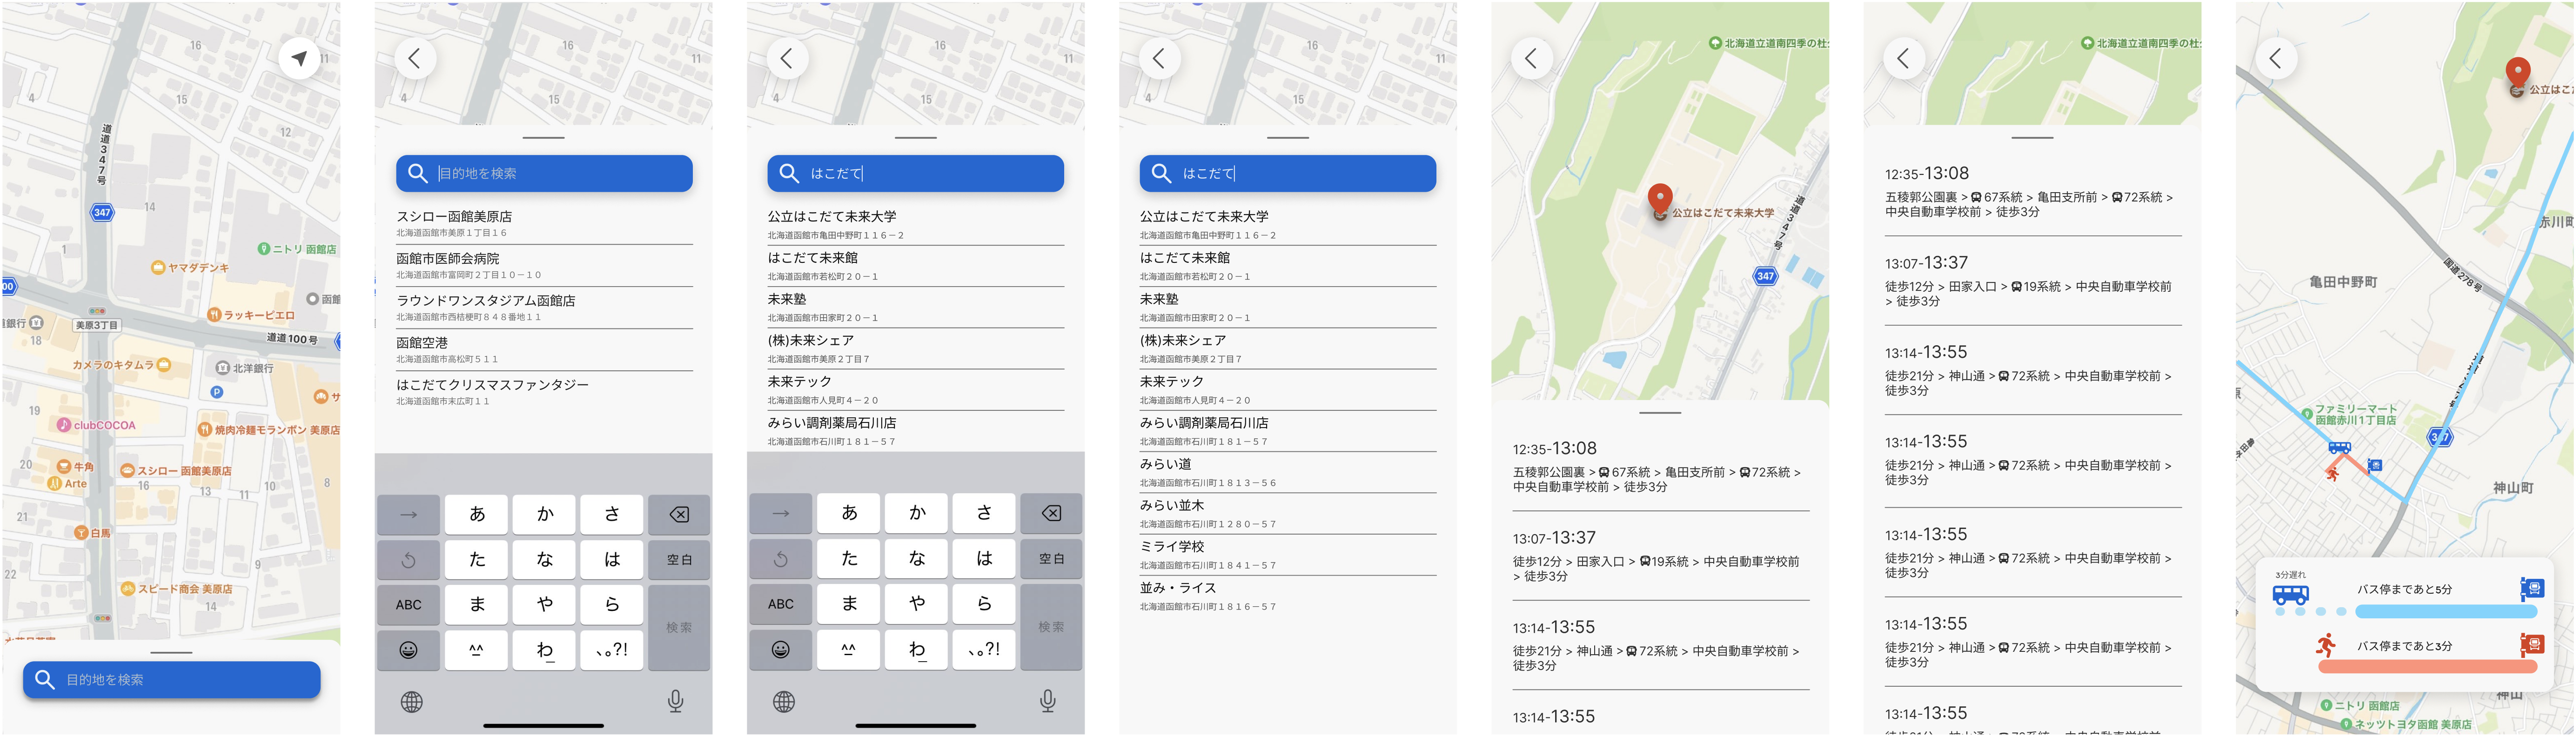
\includegraphics[width=12cm]{images/prototype_v2.png}
    \caption{プロトタイプ}
    \label{fig:prototype_v2}
\end{figure}

\subsection{フィードバック}
実際にプロジェクトメンバーにFigma\footnote{https://www.figma.com/}で作成した図2.4のプロトタイプを使用してもらった.その際たくさんの質問,指摘,意見をいただいた.一番右の画面に対して,「下のバスと人との位置関係のグラフはいるのか?」,「現在動いているバスの位置情報と自分の位置情報が分かれば大体どれくらいにバス停にいけばいいのかわかるのでは?」という意見をいただいた.それらの意見に対し,ターゲットユーザを絞ることとした.

\subsection{ターゲットユーザ}
実際に得たフィードバックから,ターゲットユーザがしっかりと定まっておらず,このアプリは何のため,誰のためのアプリなのかがわからないことに気がついた.そこでチームでもう一度ターゲットユーザについて話し合い以下のように確立させた.

\begin{quote}
    \begin{itemize}
        \item 通勤通学にバスを使っていて,バスの乗降地点が毎回同じ
        \item バスに乗り遅れたくない
        \item バス停で待ちたくない
        \item 10代後半から20代前半
    \end{itemize}
\end{quote}

\subsection{改善}
確立させたターゲットユーザに合う機能のみを実装するとしたため,合わせてプロトタイプを改善した.

図2.4のプロトタイプではユーザが毎回移動先・移動元を検索していたが,最初に登録をすることで,検索を毎回行う工程を省いた.通勤通学など,使用するバスが決まっているというユーザ像には,地点の検索は無駄な工程であった.

アプリ全体のデザインとしては,色やアイコンを改善した.具体的には,Time-Distace Viewのアイコンとその色を変更した.以前は人のアイコンが走っている人間のアイコンであり,赤色を使用していたため,焦りを与えていた.そのため,色を改善し,さらに同レベルの情報の色のコントラストを揃えた.また,Flutter\footnote{https://flutter.dev/}で開発をするにおいて,アイコンをmaterial designに統一した.

また,Time-Distance Viewについて,どの駅を使用するのか,何円かかるか,何時に到着するかなどの,ユーザが必要最低限と感じる情報を追加した.また,ウィジェット全体のサイズやレイアウトを改善した.

最後に,アプリを開いた時にランディング画面を設けることで,アプリ全体の概要や印象をユーザがわかりやすくなるよう改善した.

\begin{figure}[htbp]
    \centering
    \includegraphics[width=12cm]{images/prototype_v3.png}
    \caption{フィードバックをもとに改善したプロトタイプ}
    \label{fig:prototype_v3}
\end{figure}
\bunseki{下村蒔里萌}

\section{函館バス株式会社への訪問}
函館バス株式会社は,バス運行に関するデータを公開していないため,本グループが開発しているアプリの紹介と,データを使用させていただくために,6月16日 (金) に本グループメンバーと担当教員で函館バス株式会社に訪問した.そこで函館バス株式会社の方から「新しい観点からの機能でいい」というお言葉をいただき,データの使用の許可をいただいた.

\begin{figure}[htbp]
    \centering
    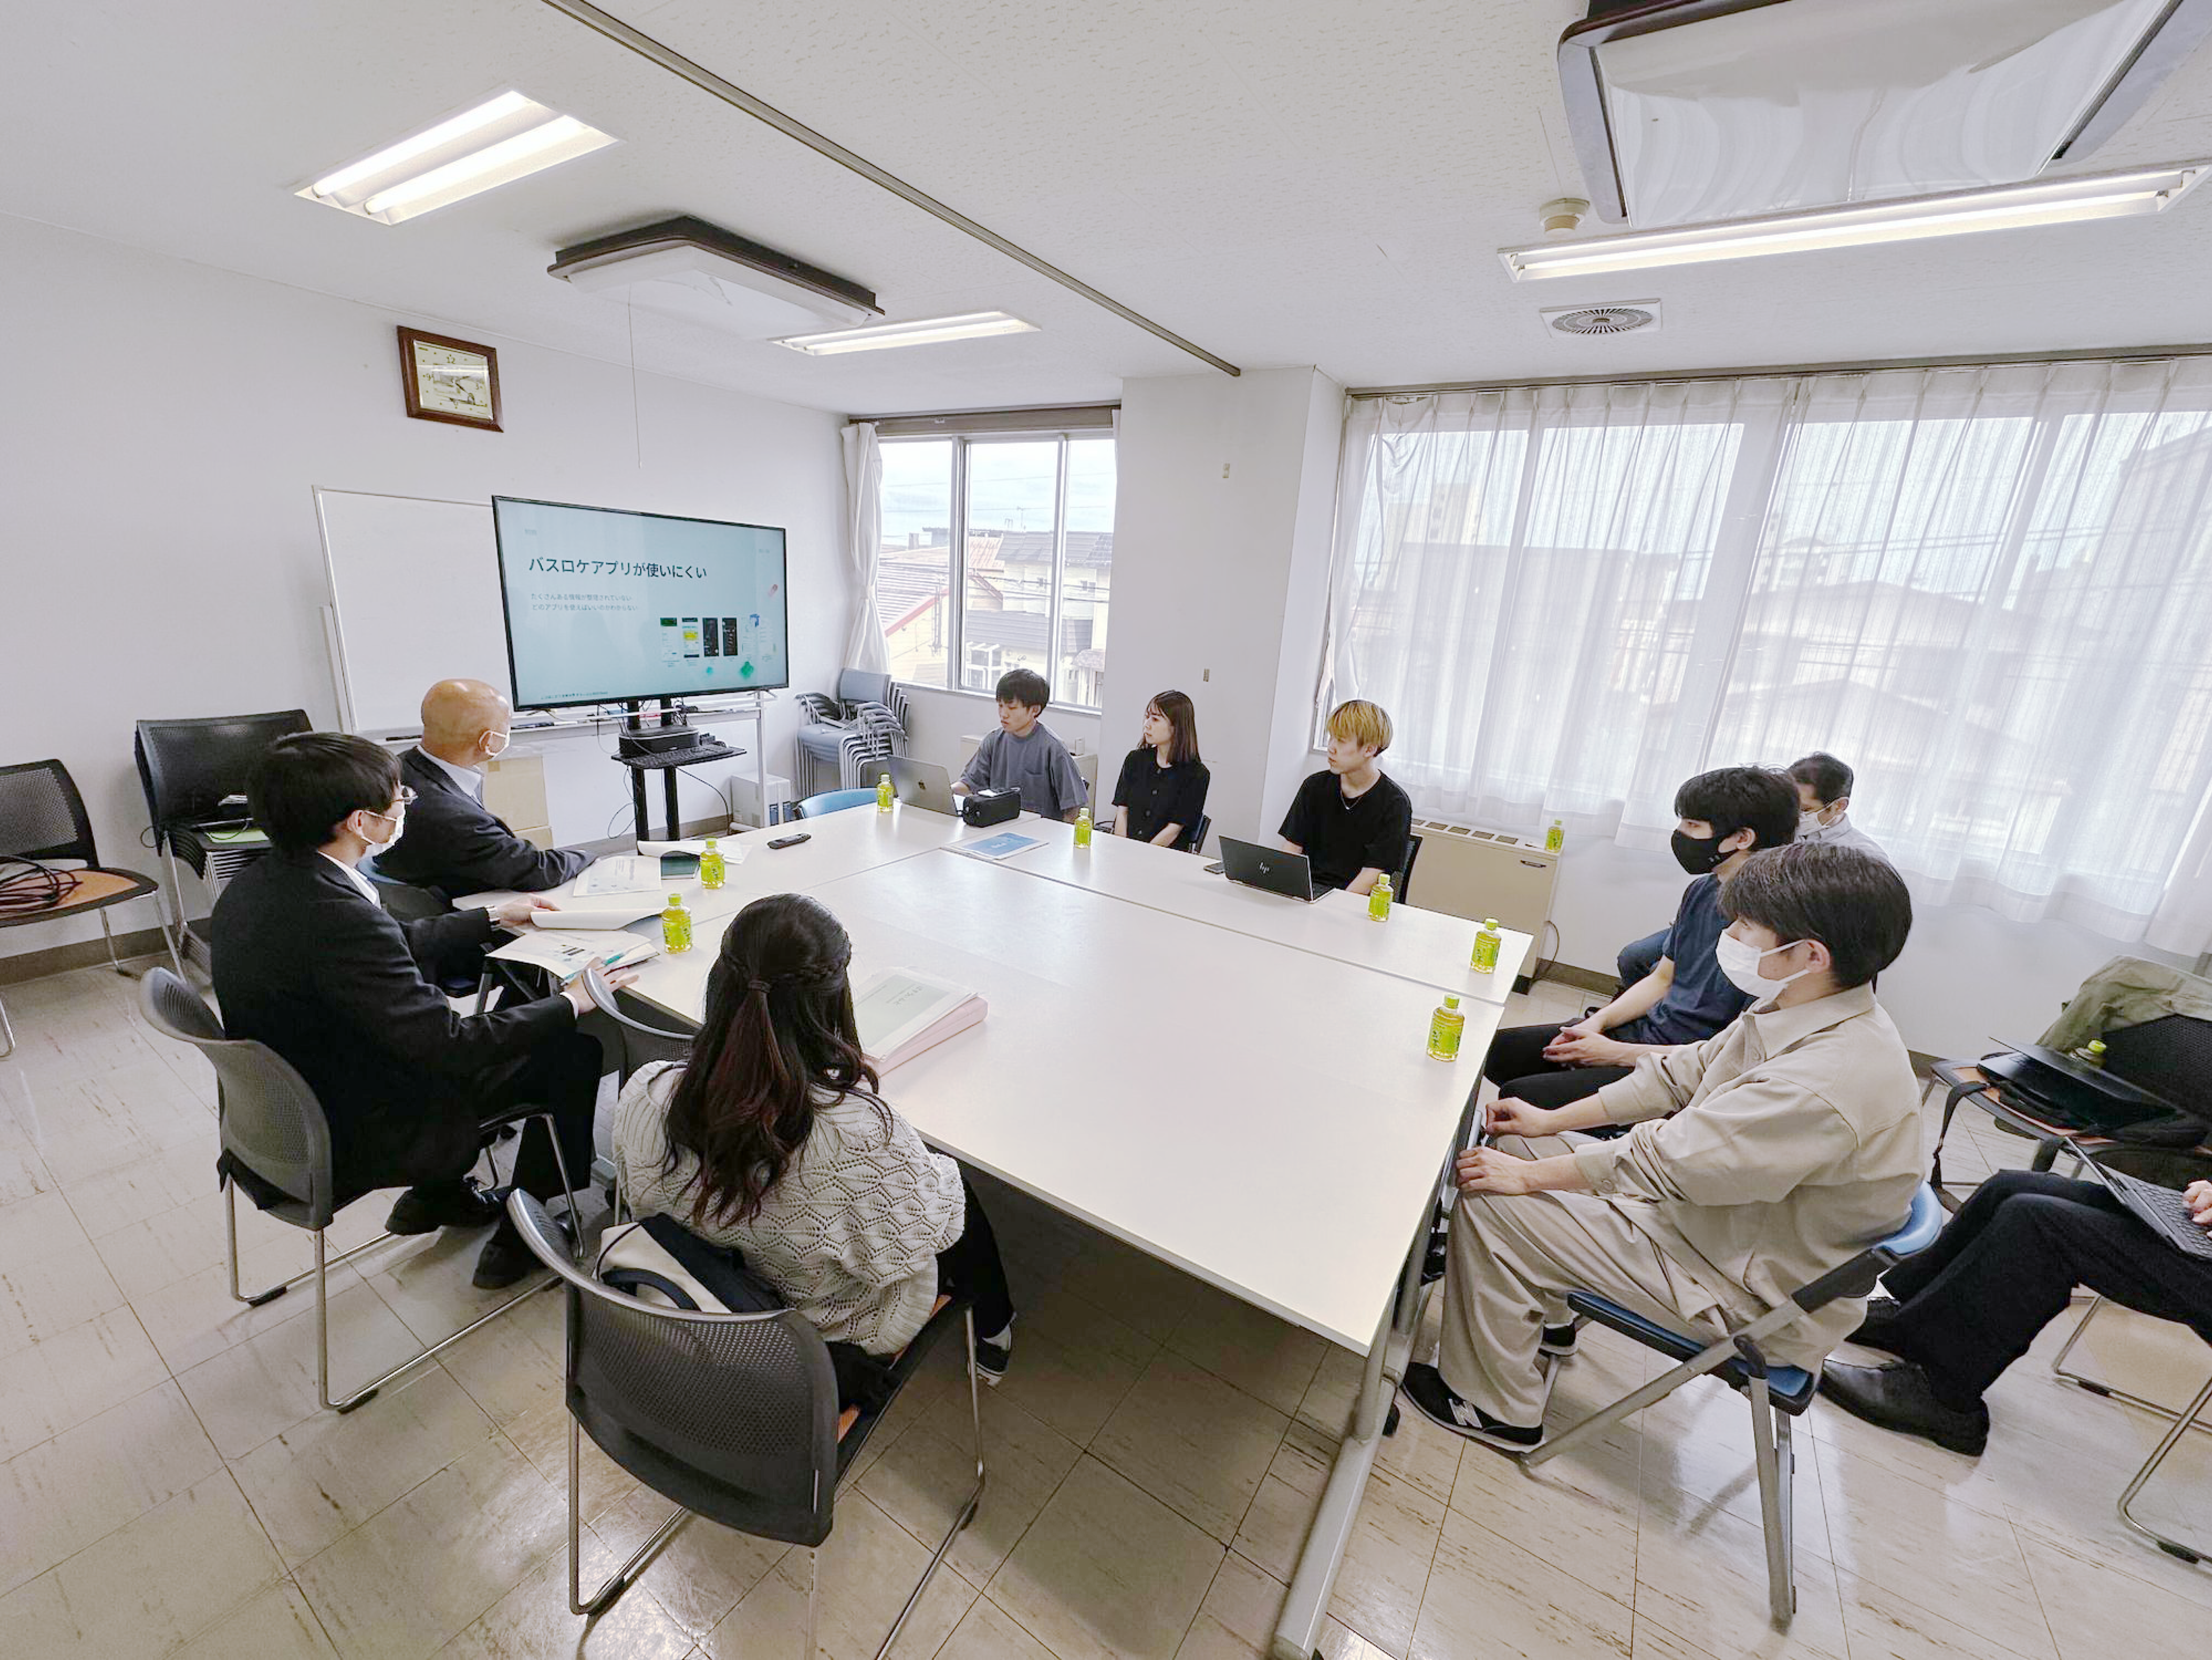
\includegraphics[width=9cm]{images/hakodate_bus.png}
    \caption{函館バス株式会社訪問時の様子}
    \label{fig:hakodate_bus}
\end{figure}
\bunseki{大津武琉}

\section{中間発表}
\subsection{中間発表資料の作成}
7月7日に行われる中間発表会に向けてスライド,メインポスター (図2.7) ,サブポスター (図2.8) を作成した.これらの資料に関して教員に繰り返しレビューをしていただき,より伝わりやすいものへと改良を重ねた.

\begin{figure}[htbp]
    \centering
    \includegraphics[width=9cm]{images/interim_poster.png}
    \caption{中間発表会メインポスター}
    \label{fig:feature_timedistanceview}
\end{figure}

\begin{figure}[htbp]
    \centering
    \includegraphics[width=9cm]{images/interim_poster_bulo.png}
    \caption{中間発表会サブポスター}
    \label{fig:interim_poster_bulo}
\end{figure}
\pagebreak
\subsection{中間発表会}
7月7日 (金) に発表会は行われた.そこで様々な質問や意見をいただいた.「首都圏と函館で同じ状況を想定していいのか?」「独自性を掲げているがUIについての独自性のみで機能についての独自性がみられない」という指摘をいただいた.これらの意見は,ターゲットユーザを絞り,合わせて実装する機能を絞った結果であると考えているため,次期バージョンにていただいた指摘をもとに改善を行う.

\begin{figure}[htbp]
    \centering
    \includegraphics[width=12cm]{images/mid_presentation.png}
    \caption{中間発表会の様子}
    \label{fig:mid_presentation}
\end{figure}
\bunseki{下村蒔里萌}
